\chapter{Perancangan}

Pada bab ini akan dijelaskan mengenai perancangan aplikasi yang dibangun meliputi perancangan interaksi antar node, perancangan aplikasi, format pesan, dan perancangan masukan dan keluaran.

\section{Perancangan Interaksi Antar Node}
\label{fungsi_interaksi}
Berikut penjelasan mengenai fungsi-fungsi aplikasi yang sudah dijelaskan pada analisis subbab \ref{fungsi}

\subsection{Diagram Sequence "Check Online Node Status"}
\begin{figure}[H] 
	\centering  
	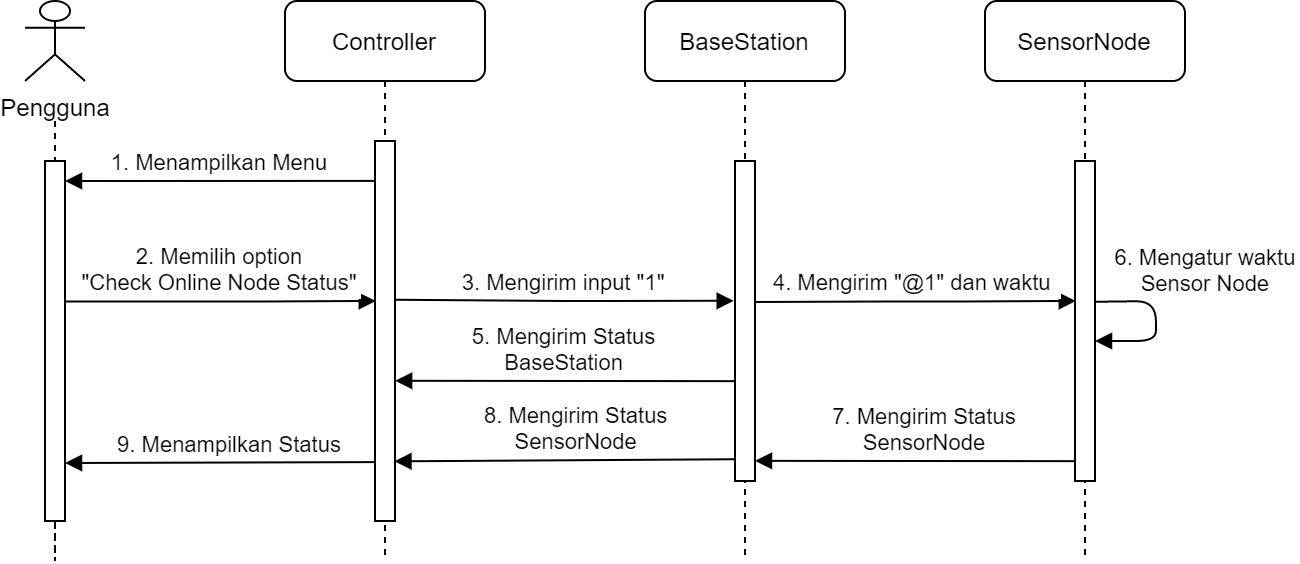
\includegraphics[scale=0.4]{Gambar/Check Online Node.jpg}  
	\caption[Diagram Sequence "Check Online Node"]{Diagram Sequence "Check Online Node"}
	\label{fig:check_online_node} 
\end{figure}

Pertama \textit{Controller} akan menampilkan menu fungsi-fungsi yang ada pada aplikasi. Kemudian pengguna akan memilih option menu "Check Online Node Status". Fungsi "Check Online Node Status" digunakan untuk menyamakan waktu dari setiap \textit{SensorNode} dan \textit{BaseStation} dengan komputer pengguna dan akan menampilkan status online dari \textit{SensorNode} dan \textit{BaseStation}. Pada saaat fungsi "Check Online Node Status" berjalan, pengguna akan memasukan kode perintah "1" dan akan dikirimkan ke \textit{BaseStation}. Setelah \textit{BaseStation} menerima kode perintah "1", BaseStation akan mengirim kode perintah "@1" ke alamat \textit{SensorNode} yang tersimpan. Setiap \textit{SensorNode} yang menerima kode perintah "@1" akan melakukan pengaturan waktu dan mengirim status \textit{online} ke BaseStation secara langsung. Setelah \textit{BaseStation} menerima status \textit{online} dari setiap \textit{SensorNode} maka \textit{BaseStation} akan meneruskan status tersebut ke \textit{Controller} dan pada \textit{Controller} akan menampilkan status \textit{online} dari \textit{SensorNode} tersebut.

\subsection{Diagram Sequence "Start Sensing"}
\begin{figure}[H] 
	\centering  
	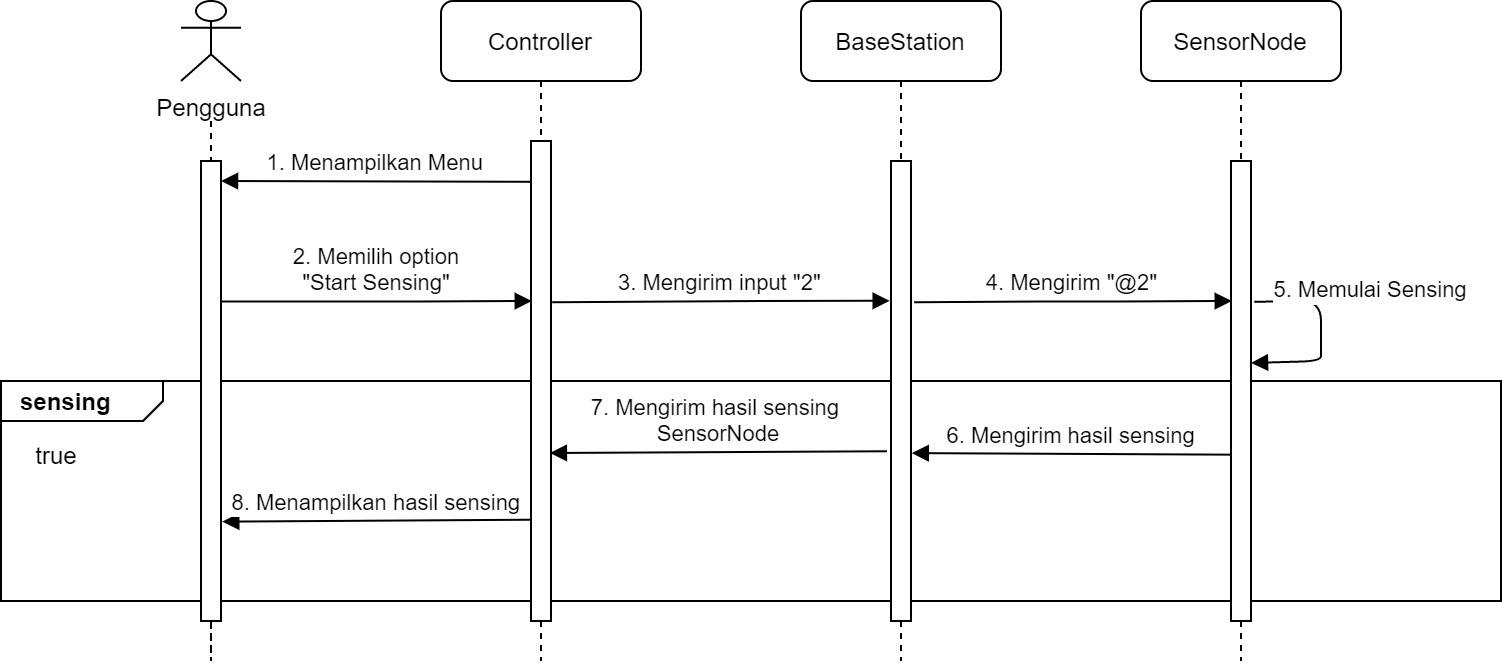
\includegraphics[scale=0.35]{Gambar/Sense.jpg}  
	\caption[Diagram Sequence "Sense"]{Diagram Sequence "Sense"}
	\label{fig:sense} 
\end{figure}

Pertama \textit{Controller} akan menampilkan menu fungsi-fungsi yang ada pada aplikasi. Setelah pengguna memilih option menu "Check Online Node Status", kemudian pengguna akan memilih option menu "Start Sensing" dengan cara memasukan kode perintah "2". Saat fungsi "Start Sensing" berjalan, Controller akan mengirimkan kode perintah "2" ke \textit{BaseStation}. Setelah kode perintah diterima oleh \textit{BaseStation}, \textit{BaseStation} akan mengirimkan kode perintah "@2" ke \textit{SensorNode}. Setiap \textit{SensorNode} yang menerima kode perintah dari \textit{BaseStation} akan melakukan \textit{sensing} dan hasilnya akan dikirimkan ke \textit{BaseStation}. Hasil sensing yang telah diterima oleh \textit{BaseStation} akan diteruskan ke \textit{Controller} dan akan ditampilkan dalam bentuk grafik.

\subsection{Diagram Sequence "Stop Sensing"}
\begin{figure}[H] 
	\centering  
	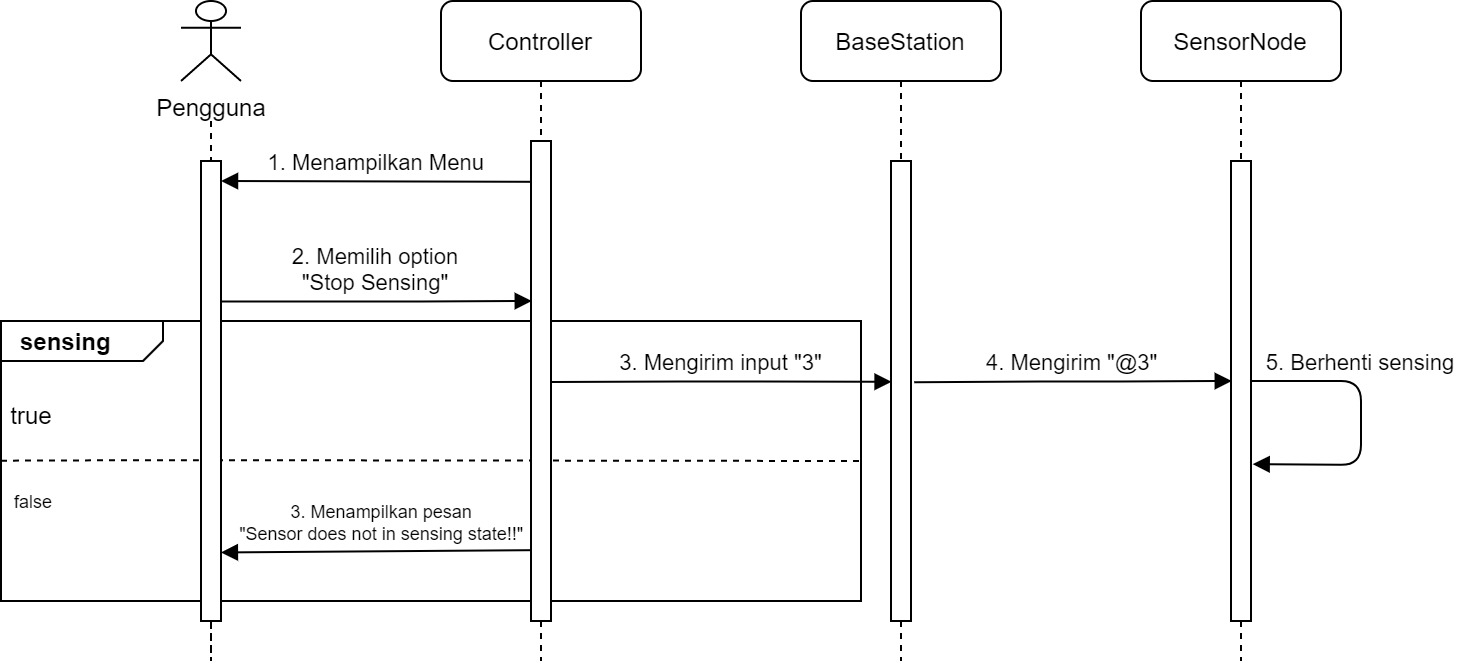
\includegraphics[scale=0.35]{Gambar/stop.jpg}  
	\caption[Diagram Sequence "Stop Sensing"]{Diagram Sequence "Stop Sensing"}
	\label{fig:stop} 
\end{figure}

Pertama \textit{Controller} akan menampilkan menu fungsi-fungsi yang ada pada aplikasi. Setelah pengguna memilih option menu "Stop Sensing". Jika \textit{SensorNode} tidak sedang dalam keadaan "Sensing" maka UserApp akan menampilkan pesan "Sensor does not in sensing state!!". Jika \textit{SensorNode} dalam keadaan "Sensing", maka \textit{Controller} akan mengirimkan kode perintah "3" ke \textit{BaseStation}. Saat \textit{BaseStation} menerima kode perintah, \textit{BaseStation} akan mengirimkan kode perintah "@3" ke \textit{SensorNode}. Setiap \textit{SensorNode} yang menerima kode perintah dari \textit{BaseStation} akan berhenti melakukan "Sensing". Saat semua \textit{SensorNode} berhenti melakukan "Sensing", \textit{Controller} akan menutup grafik hasil sense dan menampilkan pesan "Stop Sensing Done".

\subsection{Diagram Sequence "Exit Program"}
\begin{figure}[H] 
	\centering  
	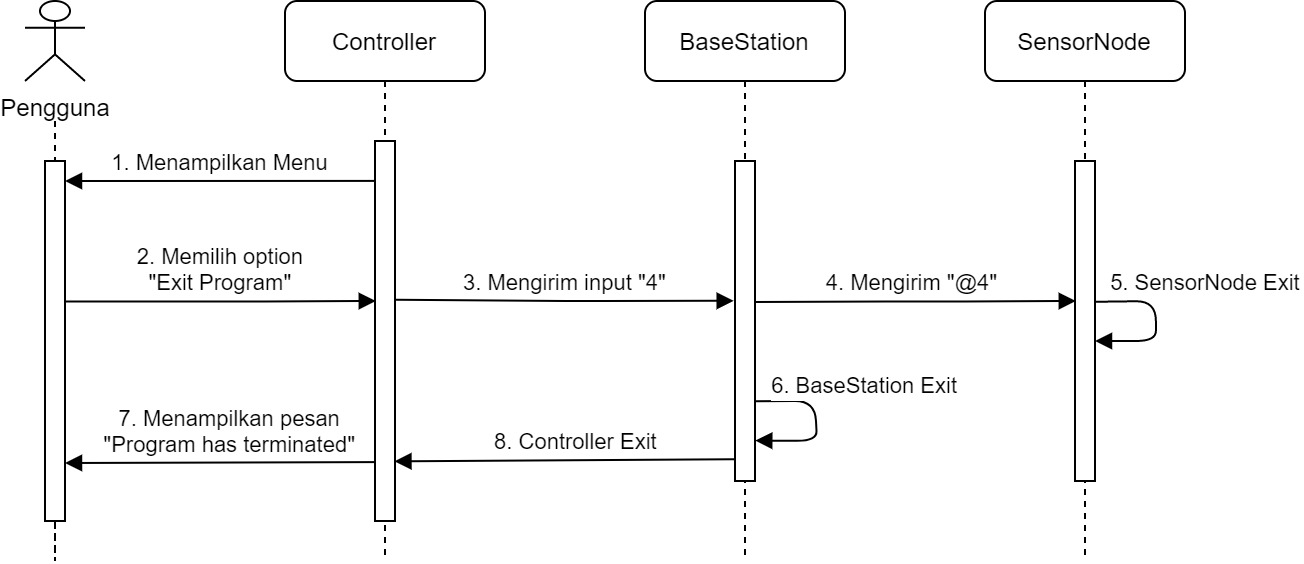
\includegraphics[scale=0.35]{Gambar/exit.jpg}  
	\caption[Diagram Sequence "Exit"]{Diagram Sequence "Exit"}
	\label{fig:exit} 
\end{figure}

Pertama \textit{Controller} akan menampilkan menu fungsi-fungsi yang ada pada aplikasi. Setelah pengguna memilih option menu "Exit Program". Saat fungsi "Exit Program" berjalan, \textit{Controller} akan mengirimkan kode peritah "4" ke \textit{BaseStation} untuk mematikan prgoram pada \textit{BaseStation}. Setelah \textit{BaseStation} menerima kode perintah, \textit{BaseStation} akan mengirimkan kode perintah "@4" ke \textit{SensorNode}. \textit{SensorNode} yang menerima kode perintah "@4" akan memberhentikan program.

\section{Perancangan Kelas Aplikasi}
Pada subbab \ref(kelas) telah dijelaskan kelas diagram sederhana untuk fungsi-fungsi pada aplikasi. Berikut versi lengkap kelas diagram dan detail dari package \textit{SensorNode}, \textit{BaseStation}, dan \textit{Controller}

\subsection{Package SensorNode}
Pada package ini terdapat kelas \textit{Accelerometer} dan \textit{SensorManager}.
\begin{figure}[H] 
	\centering  
	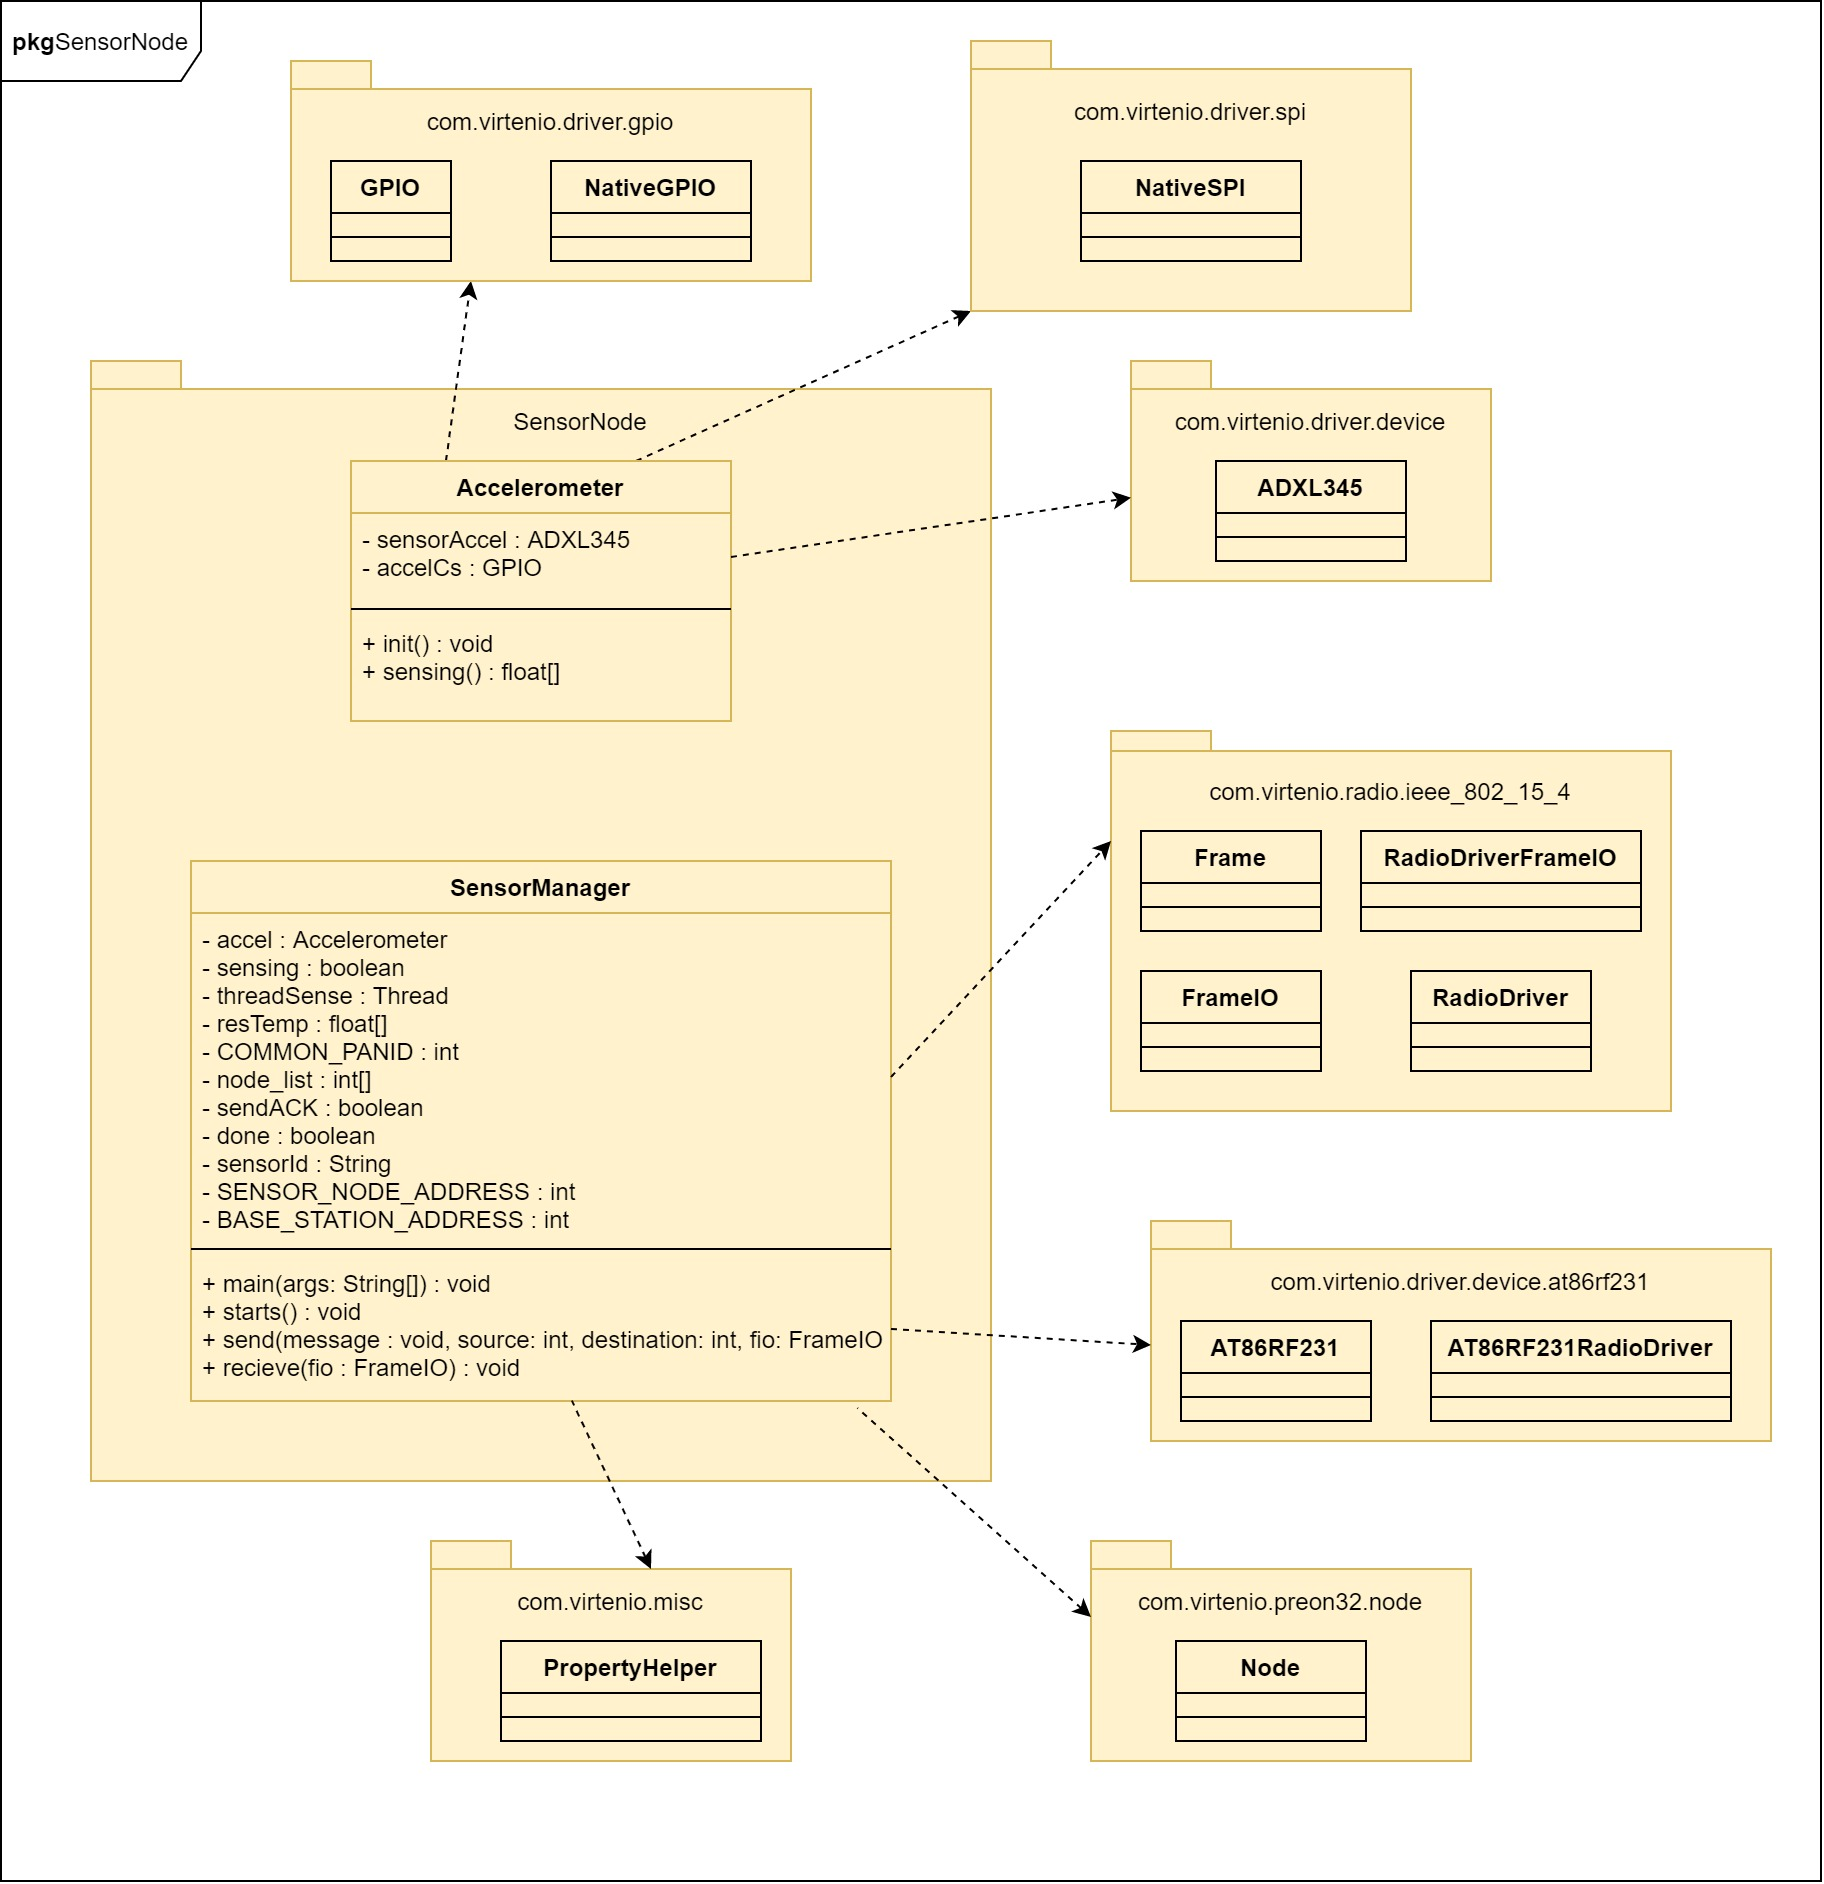
\includegraphics[scale=0.25]{Gambar/class_sensorNode.jpg}
	\caption[Kelas Diagram lengkap package SensorNode]{Kelas Diagram lengkap package SensorNode}
	\label{fig:class_sensorNode} 
\end{figure}

\subsubsection{Kelas Accelerometer}
\begin{figure}[H] 
	\centering  
	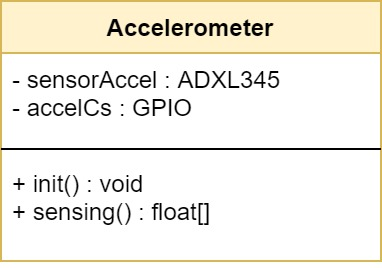
\includegraphics[scale=0.4]{Gambar/accelerometer_class.jpg}
	\caption[Perancangan Kelas Accelerometer]{Perancangan Kelas Accelerometer}
	\label{fig:accleromter_class} 
\end{figure}

Kelas ini digunakan untuk mengatur dan menginisialisasi sensor \textit{accelerometer} yang terdapat pada sensor node. Kelas ini memiliki atribut-atribut sebagai berikut:
\begin{itemize}
    \item private ADXL345 sensorAccel; 
    
    Atribut ini digunakan sebagai objek driver untuk \textit{accelerometer} ADXL345.
    \item private GPIO accelCs; 
    
    Atribut ini digunakan sebagai objek GPIO.
\end{itemize}
Metode-Metode yang terdapat pada kelas ini adalah sebagai berikut:
\begin{itemize}
    \item public void init(); 
    
    Metode ini digunakan untuk melakukan inisialisasi sensor \textit{accelerometer} ADXL345.
    \item public float[] sensing; 
    
    Metode ini digunakan untuk mendapatkan data pengukuran \textit{accelerometer} dari ADXL345.
\end{itemize}

\subsubsection{Kelas SensorManager}
\begin{figure}[H] 
	\centering  
	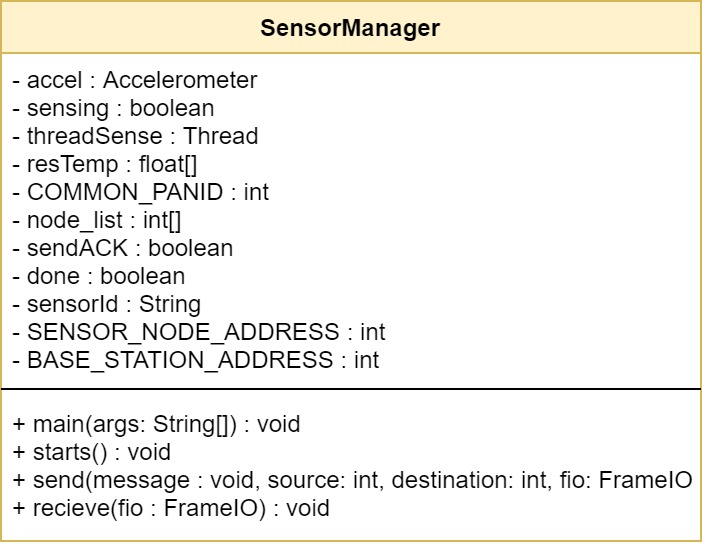
\includegraphics[scale=0.3]{Gambar/sensorManager_class.jpg}
	\caption[Perancangan Kelas SensorManager]{Perancangan Kelas SensorManager}
	\label{fig:sensorManager_class} 
\end{figure}

Kelas ini digunakan sebagai main class dari package ini. Kelas ini memiliki fungsi menerima pesan dari BaseStation dan mengirimkan hasi pengukuran ke BaseStation. Kelas ini memiliki atribut-atribut sebagai berikut:
\begin{itemize}
    \item public static final Accelerometer accel; 
    
    Atribut ini digunakan untuk menyimpan objek dari kelas Accelerometer.
    
    \item public static boolean sensing;
    
    Atribut ini digunakan untuk mengetahui kondisi sensing dari SensorNode, jika bernilai \textit{true} maka SensorNode sedang melakukan sensing.
    
    \item public Thread threadSense;
    
    Atribut ini digunakan untuk membuat \textit{thread} baru untuk melakukan sensing.
    
    \item public static float[] resTemp;
    
    Atribut ini digunakan untuk menyimpan hasil sementara dari sensing.
    
    \item public static int COMMON\_PANID;
    
    Atribut ini digunakan untuk menyimpan PANID.
    
    \item public static int[] node\_list;
    
    Atribut ini digunakan untuk menyimpan alamat-alamat dari sensor node.
    
    \item private static boolean sendACK;
    
    Atribut ini digunakan sebagai penanda bahwa SensorNode dapat mengirim data ke BaseStation. Jika bernilai true, maka SensorNode dapat mengirimkan data ke BaseStation.
    
    \item private static boolean done;
    
    Atribut ini digunakan sebagai penanda bahwa SensorNode telah mengirimkan data ke BaseStation. Jika bernilai true, maka SensorNode telah mengirimkan data ke BaseStation.
    
    \item private static final String sensorId;
    
    Atribut ini digunakan untuk menyimpan Id dari sensor node.
    
    \item private static int SENSOR\_NODE\_ADDRESS;
    
    Atribut ini digunakan untuk menyimpan alamat dari sensor node.
    
    \item private static int BASE\_STATION\_ADDRESS;
    
    Atribut ini digunakan untuk menyimpan alamat dari BaseStation.
\end{itemize}

Metode-Metode yang terdapat di kelas ini adalah sebagai berikut:
\begin{itemize}
    \item public static void main(String[] args)
    
    Metode ini digunakan sebagai metode main dari kelas SensorManager
    
    \item public static void starts();
    
    Metode ini digunakan sebagai inisialisasi radio dan memulai thread baru untuk menerima pesan dari BaseStation.
    
    \item public static void send(String message, int source, int destination, FrameIO fio);
    
    Metode ini digunakan untuk mengirim pesan ke BaseStation.
    
    \item public static void recieve(final FrameIO fio);
    
    Metode ini digunakan untuk menerima pesan dari BaseStation dan mengolah perintah yang diberikan.
\end{itemize}

\subsection{Package BaseStation}
Pada package ini terdapat kelas BaseStation

\begin{figure}[H] 
	\centering  
	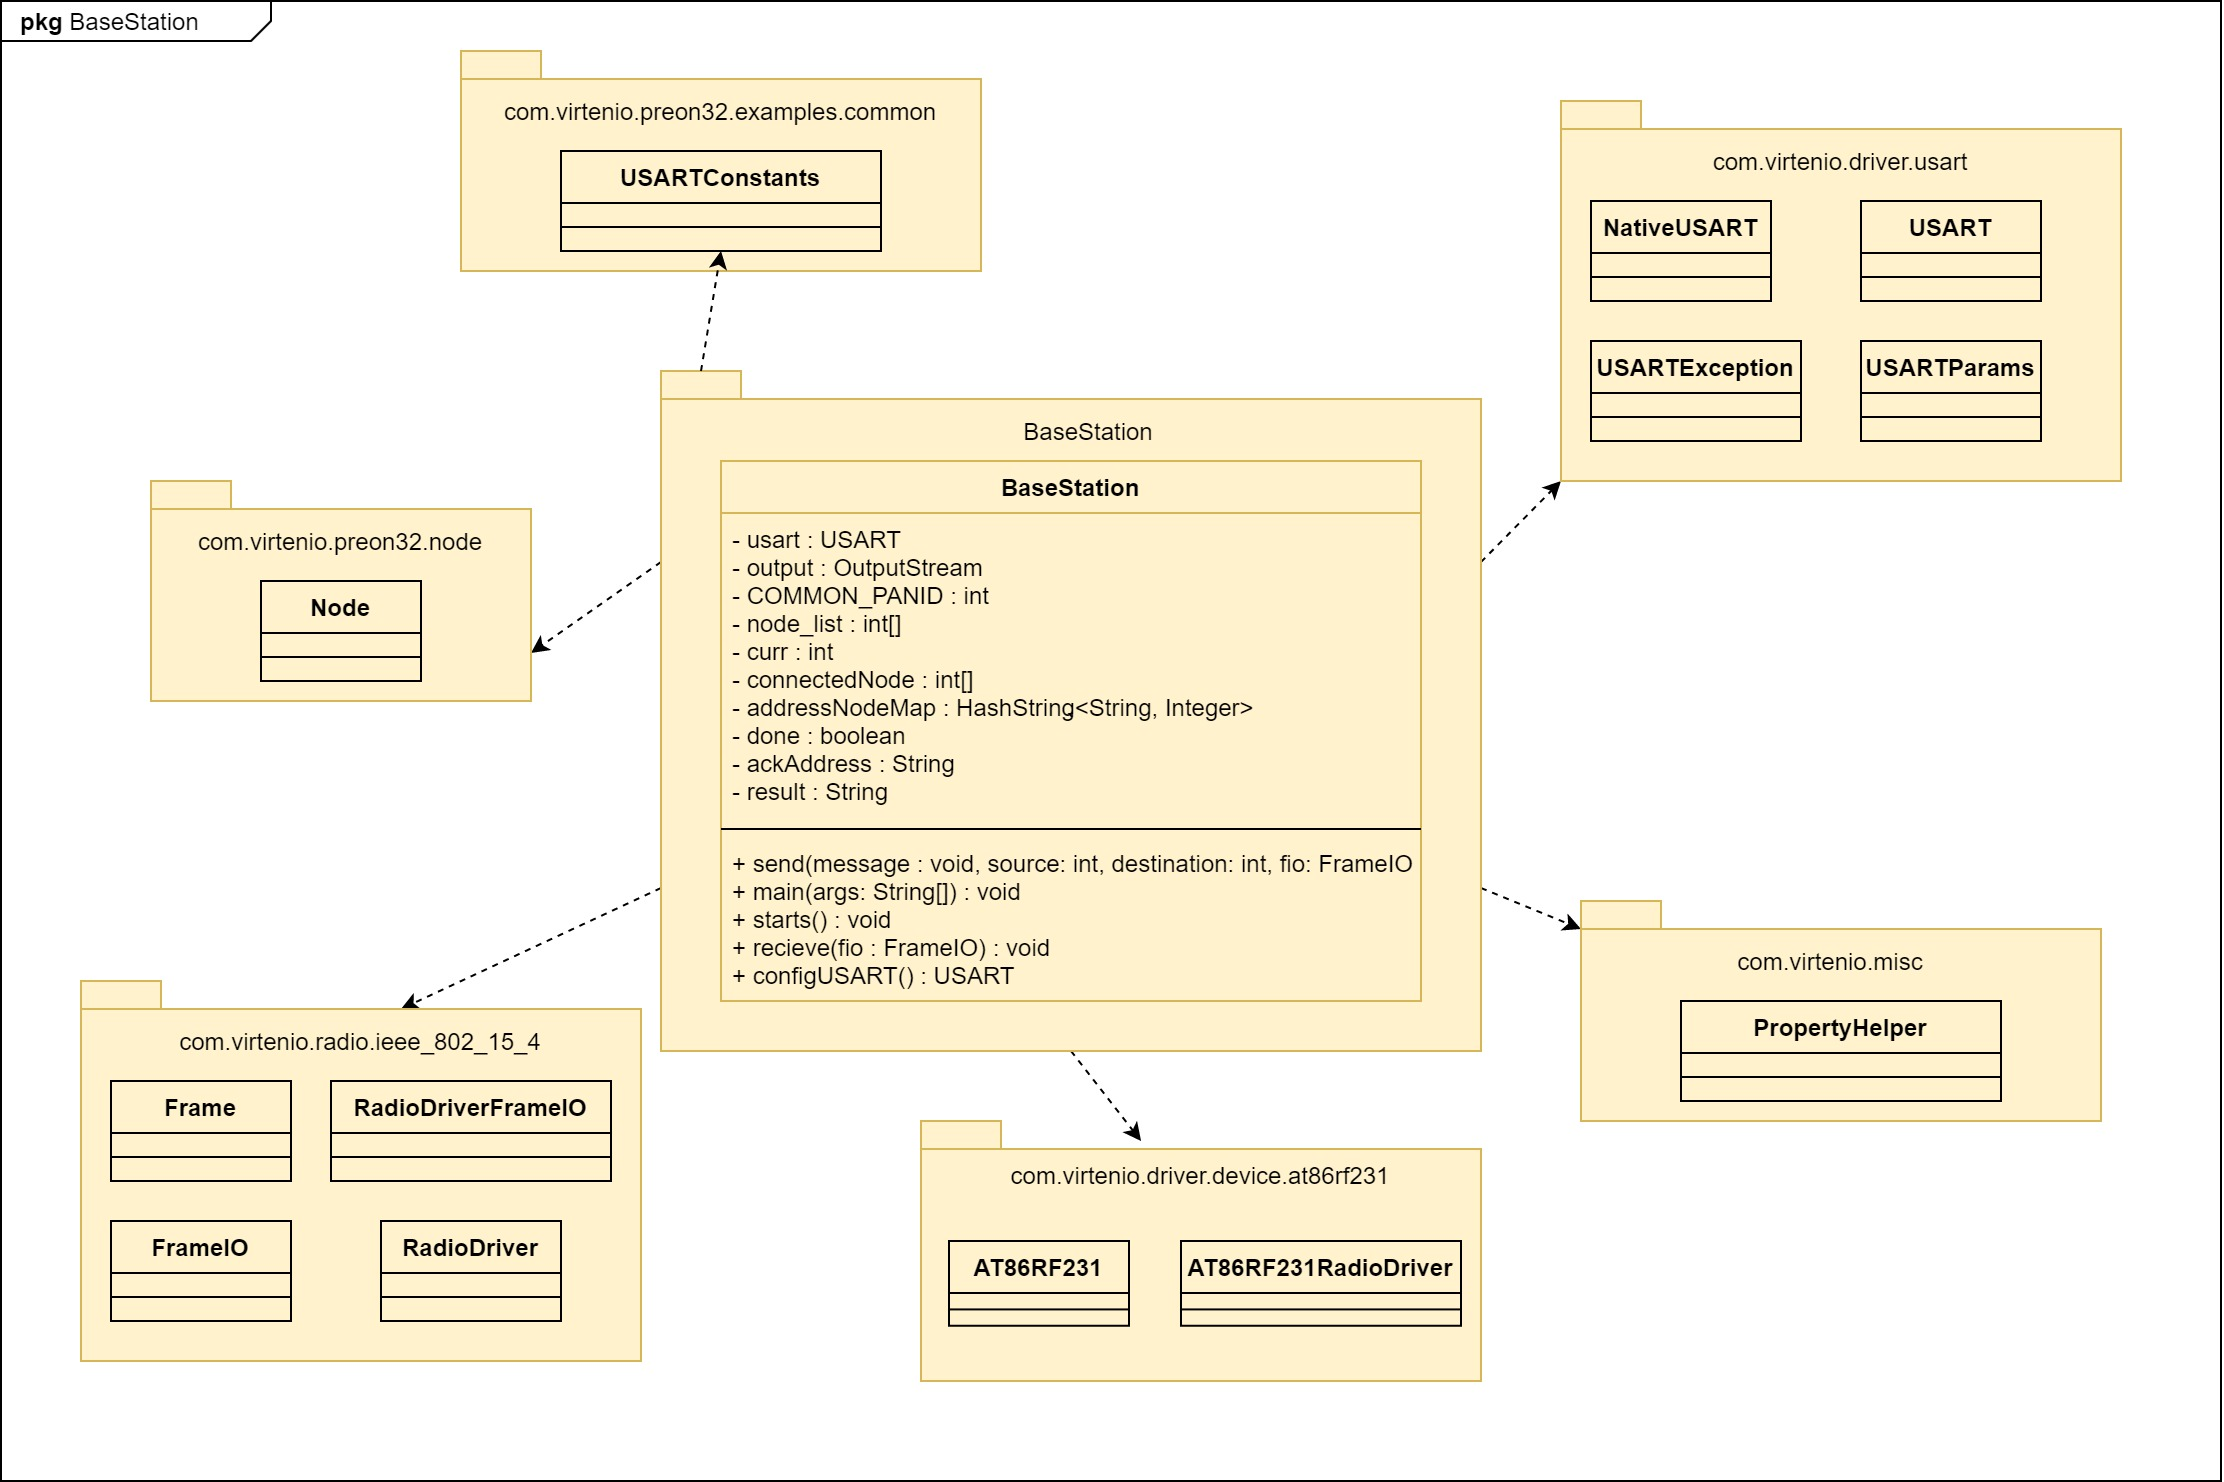
\includegraphics[scale=0.2]{Gambar/class_baseStation.jpg}
	\caption[Kelas Diagram lengkap package BaseStation]{Kelas Diagram lengkap package BaseStation}
	\label{fig:class_baseStation} 
\end{figure}


\subsubsection{Kelas BaseStation}
\begin{figure}[H] 
	\centering  
	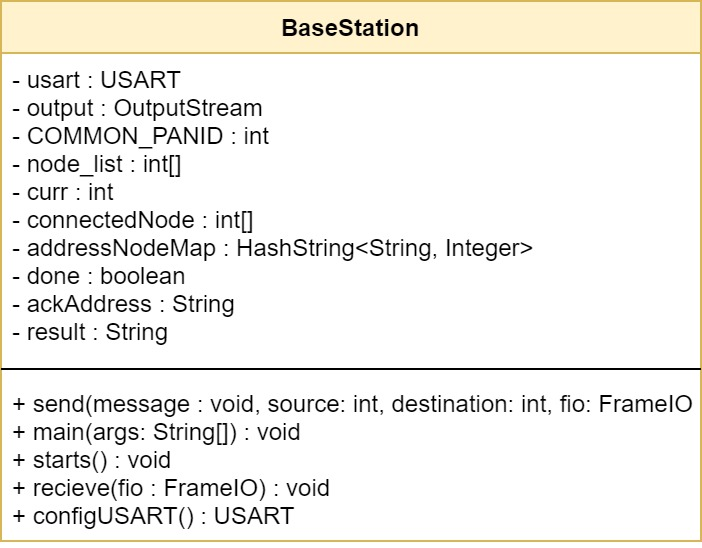
\includegraphics[scale=0.4]{Gambar/baseStation_class.jpg}
	\caption[Perancangan Kelas BaseStation]{Perancangan Kelas BaseStation}
	\label{fig:class_baseStation} 
\end{figure}
Kelas ini digunakan sebagai main class dari package BaseStation. Kelas ini berfungsi untuk menerima perintah dari Controller, meneruskan perintah ke SensorNode, menerima pesan dari SensorNode dan meneruskan pesan ke Controller. Kelas ini memiliki atribut-atribut sebagai berikut:

\begin{itemize}
    \item private static USART usart;
    
    Atribut ini digunakan mengatur usart pada BaseStation.
    
    \item private static OutputStream output;
    
    Atribut ini digunakan untuk mengatur OutputStream ke Controller.
    
    \item public static COMMON\_PANID;
    
    Atribut ini digunakan untuk menyimpan PANID.
    
    \item public static int[] node\_list;
    
    Atribut ini digunakan untuk menyimpan alamat-alamat dari sensor node.
    
    \item private static int curr;
    
    Atribut ini digunakan untuk menyimpan alamat dari BaseStation.
    
    \item private static int[] connectedNode;
    
    Atribut ini digunakan untuk menyimpan alamat sensor node yang terhubung dengan BaseStation.
    
    \item public static HashMap<String, Integer> addressNodeMap;
    
    Atribut ini digunakan untuk menyimpan alamat sensor node yang terhubung dengan BaseStation ke HashMap.
    
    \item private static boolean done;
    
    Atribut ini digunakan untuk menunjukkan apakah SensorNode telah mengirim pesan ke BaseStation.
    
    \item private static String ackAddress;
    
    Atribut ini digunakan untuk menyimpan alamat sensor node yang sedang mengirim data.
    
    \item private static String result;
    
    Atribut ini digunakan untuk menyimpan data yang terkirim oleh sensor node.
    
\end{itemize}

Metode-Metode yang terdapat pada kelas ini adalah sebagai berikut:

\begin{itemize}
    \item public static void send(String message, int source, int destination, FrameIO fio);
    
    Metode ini digunakan untuk mengirim pesan ke SensorNode.
    
    \item public static void main(String[] args);
    
    Metode ini digunakan untuk metode main dari BaseStation
    
    \item public static void starts();
    
    Metode ini digunakan untuk inisialisasi radio dan memulai thread baru untuk menerima dan mengirim pesan.
    
    \item public static void recieve(final FrameIO fio);
    
    Metode ini digunakan untuk menerima pesan yang dikirim oleh SensorNode.
    
\end{itemize}


% PACKAGE CONTROLLER
\subsection{Package Controller}
Pada package ini terdapat kelas yang dapat dilihat pada gambar dibawah:
\begin{figure}[H] 
	\centering  
	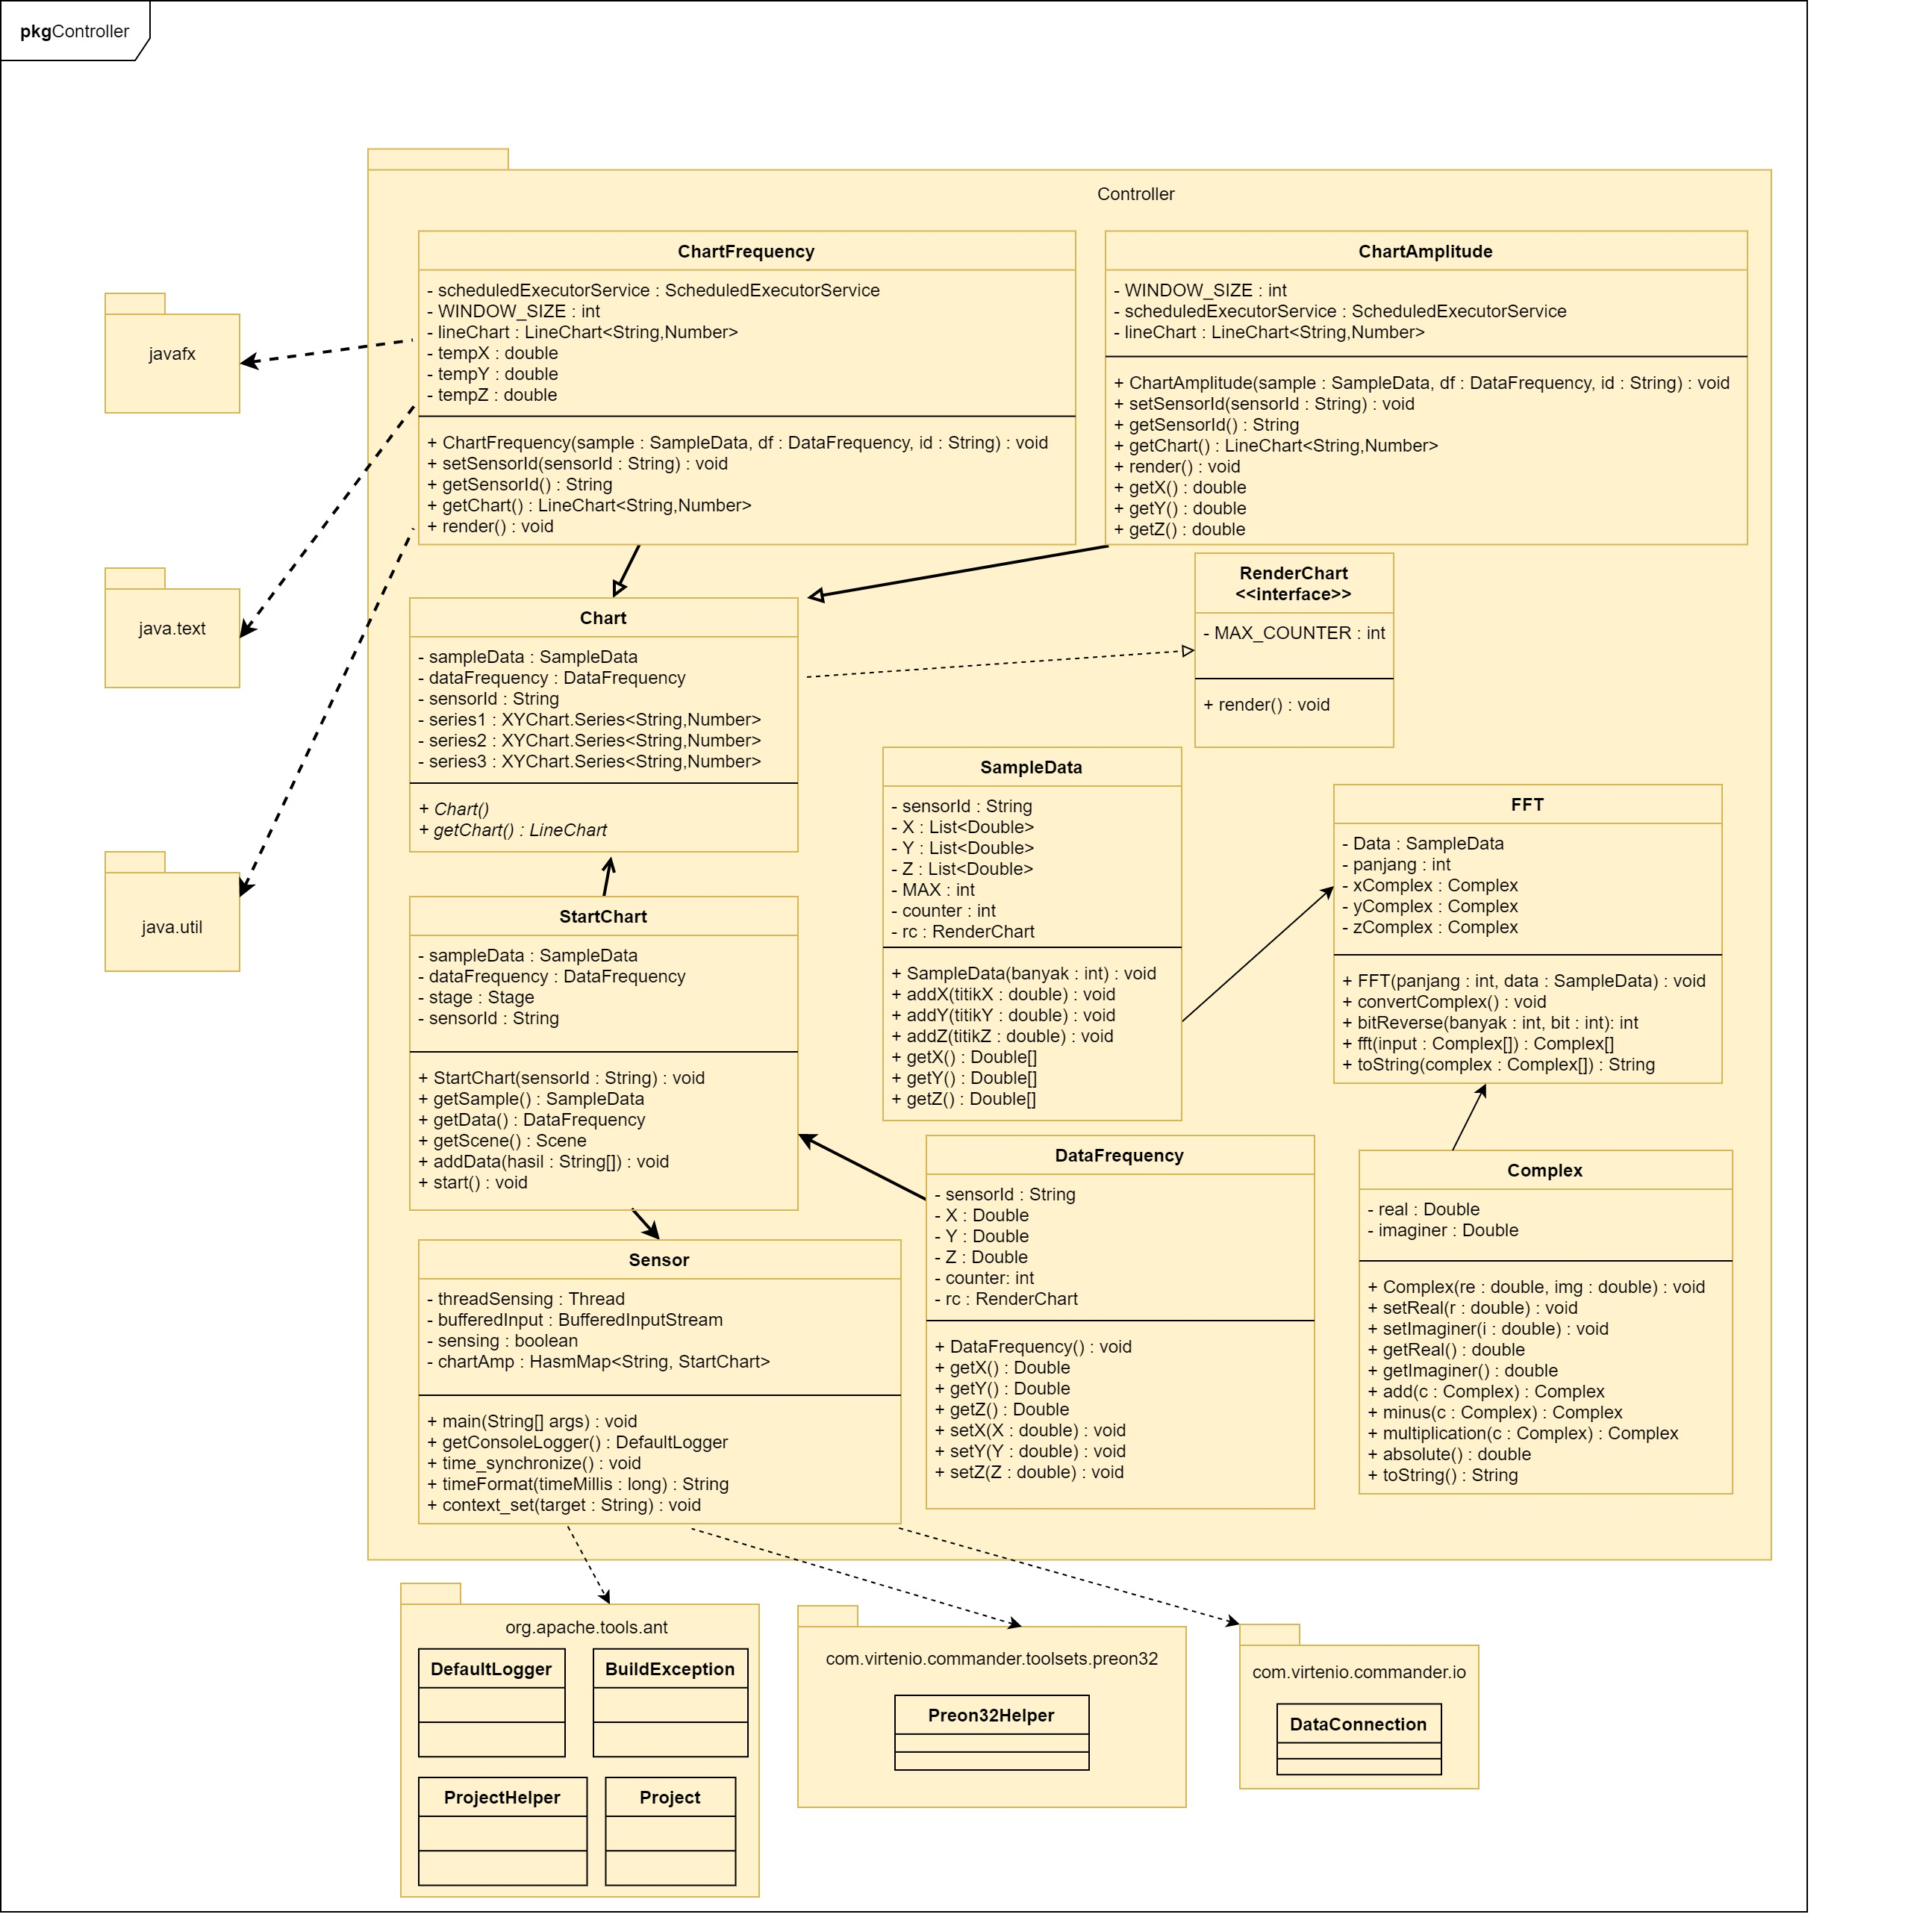
\includegraphics[scale=0.2]{Gambar/Controller Package/Controller-Controller_class.jpg}
	\caption[Kelas Diagram lengkap package Controller]{Kelas Diagram lengkap package BaseStation}
	\label{fig:controller} 
\end{figure}


% PACKAGE CONTROLLER/Complex
\subsubsection{Kelas Complex}
\begin{figure}[H] 
	\centering  
	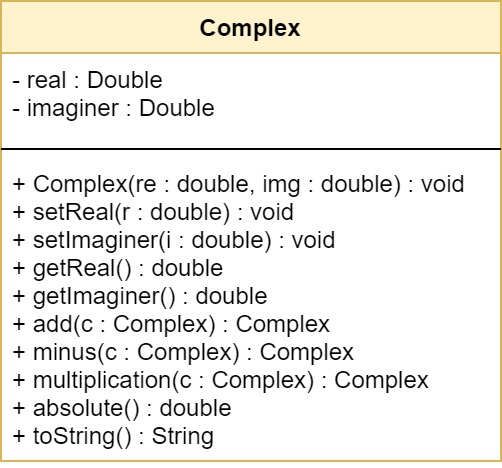
\includegraphics[scale=0.35]{Gambar/Controller Package/Controller-complex.jpg}
	\caption[Perancangan Kelas Complex]{Perancangan Kelas Complex}
	\label{fig:controller_complex} 
\end{figure}
Kelas ini digunakan sebagai objek yang mengatur dan menginisialisasi bilangan kompleks. Kelas ini memiliki atribut-atribut sebagai berikut:
\begin{itemize}
    \item public double real;
    
    Atribut ini digunakan untuk menyimpan bilangan real.
    
    \item public double imaginer;
    
    Atribut ini digunakan untuk menyimpan bilangan imajiner.
\end{itemize}

Metode-Metode yang terdapat pada kelas ini adalah sebagai berikut:
\begin{itemize}
    \item public Complex(double re, double img);
    
    Metode ini digunakan sebagai konstruktor dari kelas Complex.
    
    \item public void setReal(double r);
    
    Metode ini digunakan sebagai setter dari atribut real.
    
    \item public void setImaginer(double i);
    
    Metode ini digunakan sebagai setter dari atribut imaginer.
    
    \item public double getReal();
    
    Metode ini digunakan sebagai getter dari atribut real.
    
    \item public double getImaginer();
    
    Metode ini digunakan sebagai getter dari atribut imaginer.
    
    \item public Complex add(Complex c);
    
    Metode ini digunakan untuk melakukan penjumlahan antar bilangan kompleks.
    
    \item public Complex minus(Complex c);
    
    Metode ini digunakan untuk melakukan pengurangan antar bilangan kompleks.
    
    \item public Complex multiplication(Complex c);
    
    Metode ini digunakan untuk melakukan perkalian antar bilangan kompleks.
    
    \item public double absolute();
    
    Metode ini digunakan untuk mendapatkan nilai amplitude dari bilangan kompleks.
    
    \item public String toString();
    
    Metode ini digunakan untuk menjadikan bilangan kompleks menjadi \textit{string}.
    
\end{itemize}


% PACKAGE CONTROLLER/DataFrequency
\subsection{Kelas DataFrequency}
\begin{figure}[H] 
	\centering  
	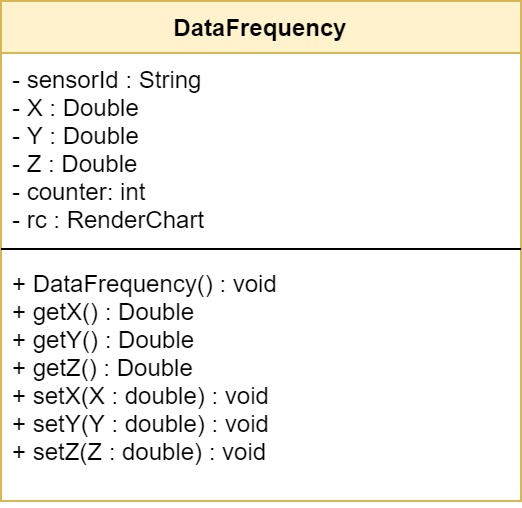
\includegraphics[scale=0.35]{Gambar/Controller Package/Controller-DataFrequency.jpg}
	\caption[Perancangan Kelas DataFrequency]{Perancangan Kelas DataFrequency}
	\label{fig:controller_datafrequency} 
\end{figure}

Kelas ini digunakan untuk menyimpan hasil perhitungan FFT. Kelas ini memiliki atribut-atribut sebagai berikut:

\begin{itemize}
    \item public String sensorId;
    
    Atribut ini digunakan untuk menyimpan nama dari sensor yang digunakan.
    
    \item public Double X;
    
    Atribut ini digunakan untuk menyimpan hasil perhitungan FFT pada sumbu X.
    
    \item public Double Y;
    
    Atribut ini digunakan untuk menyimpan hasil perhitungan FFT pada sumbu Y.
    
    \item public Double Z;
    
    Atribut ini digunakan untuk menyimpan hasil perhitungan FFT pada sumbu Z.
    
    \item private int counter=0;
    
    Atribut ini digunakan untuk menyimpan banyaknya nilai FFT yang telah disimpan dalam atribut.
    
    \item private RenderChart rc;
    
    Atribut ini digunakan untuk menyimpan objek dari kelas RenderChart.
\end{itemize}

Metode-metode yang terdapat pada kelas ini adalah sebagai berikut:
\begin{itemize}
    \item public DataFrequency();
    
    Metode ini merupakan konstruktor dari kelas DataFrequency.
    
    \item public void setRender(RenderChart rc);
    
    Metode ini merupakan \textit{setter} dari atribut rc.
    
    \item public Double getX();
    
    Metode ini merupakan \textit{getter} dari atribut X.
    
     \item public Double getY();
    
    Metode ini merupakan \textit{getter} dari atribut Y.
    
    \item public Double getZ();
    
    Metode ini merupakan \textit{getter} dari atribut Z.
    
    \item public void setX();
    
    Metode ini merupakan \textit{setter} dari atribut X.
    
    \item public void setY();
    
    Metode ini merupakan \textit{setter} dari atribut Y.
    
    \item public void setY();
    
    Metode ini merupakan \textit{setter} dari atribut Z.
    
\end{itemize}


% PACKAGE CONTROLLER/FFT
\subsubsection{Kelas FFT}
\begin{figure}[H] 
	\centering  
	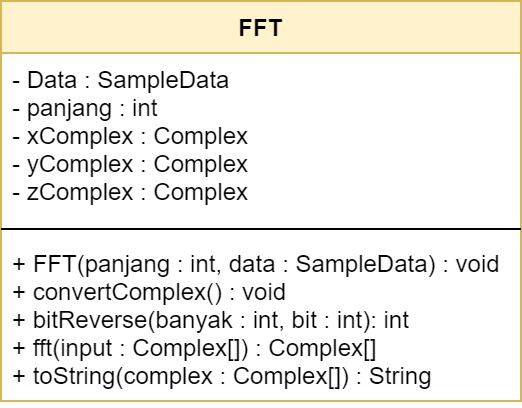
\includegraphics[scale=0.35]{Gambar/Controller_fft.jpg}
	\caption[Perancangan Kelas FFT]{Perancangan Kelas FFT}
	\label{fig:controller_fft} 
\end{figure}

Kelas ini digunakan untuk melakukan komputasi FFT dari input bilangan kompleks. Kelas ini memiliki atribut-atribut sebagai berikut:
\begin{itemize}
    \item public SampleData data;
    
    Atribut ini digunakan untuk menyimpan sampel data.
    
    \item public int panjang;
    
    Atribut ini digunakan untuk menyimpan panjang dari algoritma FFT.
    
    \item public Complex xComplex;
    
    Atribut ini digunakan untuk menyimpan nilai bilangan kompleks pada sumbu x.
    
    \item public Complex yComplex;
    
    Atribut ini digunakan untuk menyimpan nilai bilangan kompleks pada sumbu y.
    
    \item public Complex zComplex;
    
    Atribut ini digunakan untuk menyimpan nilai bilangan kompleks pada sumbu z.
\end{itemize}

Metode-metode yang terdapat pada kelas ini adalah sebagai berikut:
\begin{itemize}
    \item public FFT(int panjang, SampleData data);
    
    Metode ini digunakan sebagai konstruktor dari kelas FFT.
    
    \item public void convertComplex();
    
    Metode ini digunakan untuk menyimpan hasil sensing ke dalam bilangan kompleks.
    
    \item public int bitReverse(int banyak, int bit);
    
    Metode ini digunakan untuk melakukan \textit{bit reverse} pada bilangan masukan.
    
    \item public Complex[] fft(Complex[] input);
    
    Metode ini digunakan untuk melakukan komputasi algoritma FFT.
    
    \item public String toString(Complex[] complex);
    
    Metode ini digunakan untuk mengubah bilangan kompleks menjadi \textit{String}.
\end{itemize}


% PACKAGE CONTROLLER/RenderChart
\subsection{Kelas RenderChart}
\begin{figure}[H] 
	\centering  
	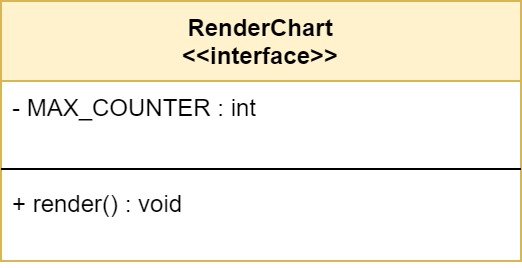
\includegraphics[scale=0.35]{Gambar/Controller Package/Controller-RenderChart.jpg}
	\caption[Perancangan Kelas RenderChart]{Perancangan Kelas RenderChart}
	\label{fig:controller_startChart} 
\end{figure}

Kelas ini merupakan \textit{interface class} yang akan digunakan oleh kelas StartChart\ref{fig:controller_startChart} untuk melakukan visualisasi grafik. Pada kelas ini, terdapat atribut beserta metode yang akan digunakan oleh kelas lain adalah sebagai berikut:

\begin{itemize}
    \item public static final int MAX\_COUNTER=64;
    
    Atribut digunakan untuk membatasi limitasi banyak data yang akan digunakan untuk melakukan perhitungan.
    
    \item public void render();
    
    Metode ini digunakan untuk melakukan proses visualisasi dalam grafik.
\end{itemize}


% PACKAGE CONTROLLER/STARTCHART
\subsection{Kelas StartChart}
\begin{figure}[H] 
	\centering  
	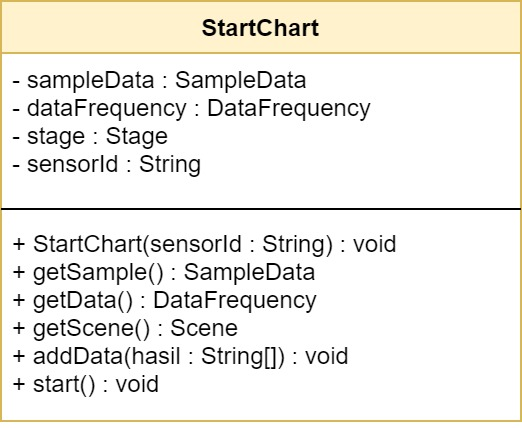
\includegraphics[scale=0.35]{Gambar/Controller Package/Controller-StartChart.jpg}
	\caption[Perancangan Kelas StartChart]{Perancangan Kelas StartChart}
	\label{fig:controller_startChart} 
\end{figure}

Kelas ini digunakan untuk melakukan visualisasi grafik. Kelas ini memiliki atribut-atribut sebagai berikut:
\begin{itemize}
    \item public ArrayList<Chart> charts;
    
    Atribut ini digunakan untuk menyimpan grafik yang akan ditampilkan secara visual.
    
    \item private SampleData data;
    
    Atribut ini digunakan untuk menyimpan sampel data.
    
    \item private DataFrequency dataFrequency;
    
    Atribut ini digunakan untuk menyimpan nilai frekuensi hasil FFT.
    
    \item private Stage stage;
    
    Atribut ini digunakan untuk membuat objek Stage yang digunakan untuk melakukan visualisasi grafik.
    
    \item private String sensorId;
    
    Atribut ini digunakan untuk menyimpan id dari sensor.
\end{itemize}

Metode-metode yang terdapat pada kelas ini adalah sebagai berikut:
\begin{itemize}
    \item public StartChart(String sensorId);
    
    Metode ini digunakan sebagai konstruktor dari kelas StartChart.
    
    \item public SampleData getSample();
    
    Metode ini digunakan untuk mendapatkan objek dari kelas SampleData.
    
    \item public DataFrequency getData();
    
    Metode ini digunakan untuk mendapatkan objek dari kelas DataFrequency.
    
    \item public Scene getScene();
    
    Metode ini digunakan mengatur bagaimana grafik yang akan ditampilkan akan terlihat.
    
    \item public void addData();
    
    Metode ini digunakan untuk menyimpan nilai amplitudo serta nilai FFT yang telah didapatkan setelah melakukan perhitungan.
    
    \item public void start();
    
    Metode ini digunakan untuk menjalankan kelas ini sehingga grafik yang akan divisualisasikan berhasil terlihat.
\end{itemize}


% PACKAGE CONTROLLER/CHART
\subsection{Kelas Chart}
\begin{figure}[H] 
	\centering  
	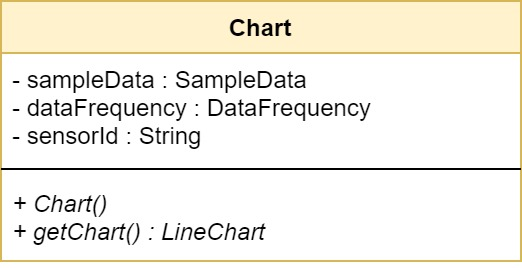
\includegraphics[scale=0.35]{Gambar/Controller_Charts.jpg}
	\caption[Perancangan Kelas Chart]{Perancangan Kelas Chart}
	\label{fig:controller_chart} 
\end{figure}

Kelas ini merupakan \textit{abstract class} yang merupakan \textit{implements} dari kelas RenderChart. Kelas ini akan digunakan oleh kelas lain untuk melakukan visualisasi. Kelas ini memiliki atribut-atribut sebagai berikut:
\begin{itemize}
    \item public SampleData sampleData;
    
    Atribut ini digunakan sebagai objek dari kelas SampleData.
    
    \item public DataFrequency dataFrequency;
    
    Atribut ini digunakan sebagai objek dari kelas DataFrequency.
    
    \item public String sensorId;
    
    Atribut ini digunakan untuk menyimpan nama dari sensor yang digunakan.
    
    \item XYChart.Series<String,Number> series1 = new XYChart.Series<>();
    
    Atribut ini digunakan untuk menginisialisasi kelas XYChart yang akan digunakan untuk membuat sumbu X pada grafik yang akan divisualisasikan.
    
    \item XYChart.Series<String,Number> series2 = new XYChart.Series<>();
    
    Atribut ini digunakan untuk menginisialisasi kelas XYChart yang akan digunakan untuk membuat sumbu Y pada grafik yang akan divisualisasikan.
    
    \item XYChart.Series<String,Number> series3 = new XYChart.Series<>();
    
    Atribut ini digunakan untuk menginisialisasi kelas XYChart yang akan digunakan untuk membuat sumbu Z pada grafik yang akan divisualisasikan.
    
    \item final SimpleDateFormat simpleDateFormat = new SimpleDateFormat("HH:mm:ss");
    
    Atribut ini digunakan untuk menyimpan format waktu yang akan ditampilkan pada grafik.
\end{itemize}

Metode yang terdapat pada kelas ini adalah sebagai berikut:
\begin{itemize}
    \item public abstract LineChart getChart();
    
    Metode ini merupakan metode \textit{abstract} yang akan digunakan oleh kelas lain yang berfungsi untuk mendapatkan grafik yang akan ditampilkan.
\end{itemize}


% PACKAGE CONTROLLER/CHARTAMPLITUDE
\subsection{Kelas ChartAmplitude}
\begin{figure}[H] 
	\centering  
	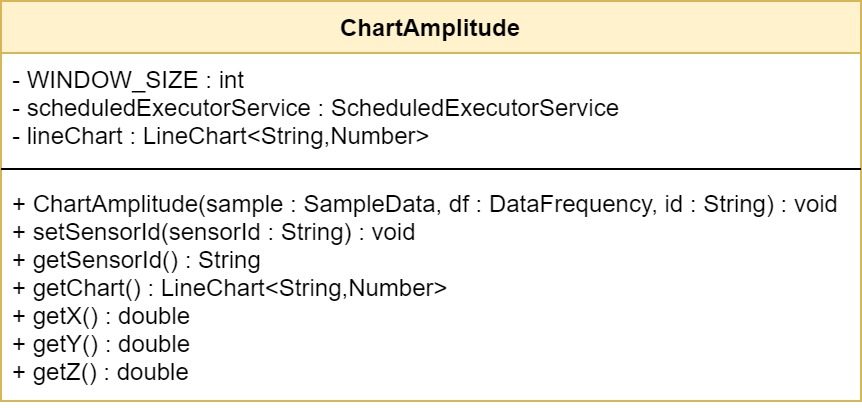
\includegraphics[scale=0.35]{Gambar/Controller_ChartAmplitude.jpg}
	\caption[Perancangan Kelas ChartAmplitude]{Perancangan Kelas ChartAmplitude}
	\label{fig:controller_chartAmplitude} 
\end{figure}

Kelas ini merupakan kelas yang akan digunakan untuk menampilkan grafik nilai amplitudo dari sensor. Kelas ini memiliki atribut-atribut sebagai berikut:

\begin{itemize}
    \item final int WINDOW\_SIZE=10;
    
    Atribut ini digunakan untuk menentukan berapa banyak nilai yang akan ditampilkan dalam grafik, dalam hal ini banyak nilai yang akan ditampilkan adalah 10 nilai.
    
    \item private ScheduledExecutorService scheduledExecutorService;
    
    Atribut ini digunakan untuk melakukan update terhadap nilai-nilai amplitudo yang akan ditampilkan ke dalam grafik.
    
    \item public LineChart<String,Number> lineChart;
    
    Atribut ini digunakan untuk menyimpan grafik dari amplitudo ini dalam bentuk \textit{line chart}.
    
\end{itemize}

Metode-metode yang terdapat pada kelas ini adalah sebagai berikut:

\begin{itemize}
    \item public ChartAmplitude(SampleData sample, DataFrequency df, String id);
    
    Metode ini digunakan sebagai konstruktor pada kelas ChartAmplitude.
    
    \item public void setSensorId(String sensorId);
    
    Metode ini merupakan \textit{setter} dari atribut sensorId.
    
    \item public String getSensorId();
    
    Metode ini merupakan \textit{getter} dari atribut sensorId.
    
    \item public LineChart<String, Number> getChart();
    
    Metode ini digunakan untuk membuat komponen-komponen yang akan digunakan untuk melakukan visualisasi nilai amplitudo.
    
    \item public void render();
    
    Metode ini digunakan untuk memasukan nilai-nilai amplitudo yang akan ditampilkan ke dalam bentuk grafik.
    
    \item public double getX();
    
    Metode ini digunakan untuk mendapatkan nilai rata-rata amplitudo pada sumbu X.
    
     \item public double getY();
    
    Metode ini digunakan untuk mendapatkan nilai rata-rata amplitudo pada sumbu Y.
    
     \item public double getZ();
    
    Metode ini digunakan untuk mendapatkan nilai rata-rata amplitudo pada sumbu Z.
\end{itemize}


% PACKAGE CONTROLLER/CHARTFREQUENCY
\subsection{Kelas ChartFrequency}
\begin{figure}[H] 
	\centering  
	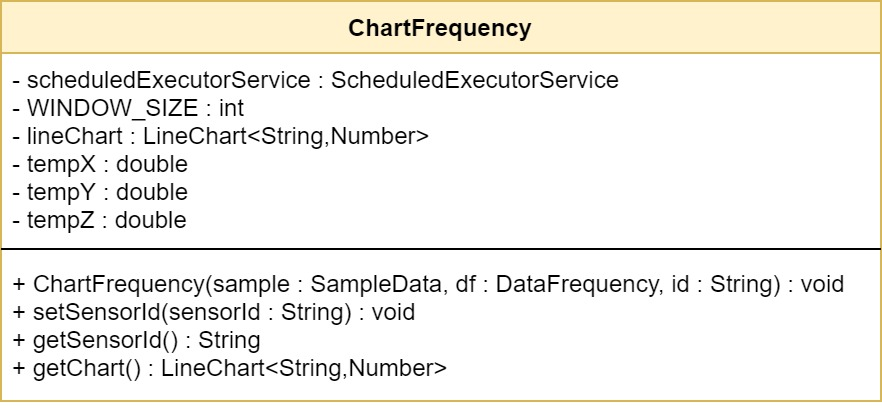
\includegraphics[scale=0.35]{Gambar/Controller_ChartFrequency.jpg}
	\caption[Perancangan Kelas ChartFrequency]{Perancangan Kelas ChartFrequency}
	\label{fig:controller_chartFrequency} 
\end{figure}

Kelas ini merupakan kelas yang akan digunakan untuk menampilkan grafik nilai frekeunsi dari sensor. Kelas ini memiliki atribut-atribut sebagai berikut:

\begin{itemize}
    \item private ScheduledExecutorService scheduledExecutorService;
    
    Atribut ini digunakan unutk melakukan update terhadap nilai-nilai frekuensi yang akan ditampilkan ke dalam grafik.
    
    \item final int WINDOW\_SIZE=10;
    
    Atribut ini digunakan untuk menentukan berapa banyak nilai yang akan ditampilkan dalam grafik, dalam hal ini banyak nilai yang akan ditampilkan adalah 10 nilai.
    
    \item public LineChart<String,Number> lineChart;
    
    Atribut ini digunakan untuk menyimpan grafik dari frekuensi ke dalam bentuk \textit{line chart}.
    
    \item public static double tempX;
    
    Atribut ini digunakan untuk menyimpan nilai hasil perhitungan FFT pada sumbu X.
    
    \item public static double tempY;
    
    Atribut ini digunakan untuk menyimpan nilai hasil perhitungan FFT pada sumbu Y.
    
    \item public static double tempZ;
    
    Atribut ini digunakan untuk menyimpan nilai hasil perhitungan FFT pada sumbu Z.
\end{itemize}

Metode-metode yang terdapat pada kelas ini adalah sebagai berikut:
\begin{itemize}
    \item public ChartFrequency(SampleData sample, DataFrequency df, String id);
    
    Metode ini digunakan sebagai konstruktor pada kelas ChartFrequency.
    
    \item public void setSensorId(String sensorId);
    
    Metode ini merupakan \textit{setter} dari atribut sensorId.
    
    \item public String getSensorId();
    
    Metode ini merupakan \textit{getter} dari atribut sensorId.
    
    \item public LineChart<String,Number> getChart();
    
    Metode ini digunakan untuk membuat komponen-komponen yang akan digunakan untuk melakukan visualisasi nilai frekuensi.
    
    \item public void render();
    
    Metode ini digunakan untuk memasukkan nilai-nilai frekuensi hasil perhitungan yang akan ditampilkan dalam bentuk grafik.

\end{itemize}


% PACKAGE CONTROLLER/SampleData
\subsubsection{Kelas SampleData}
\begin{figure}[H] 
	\centering  
	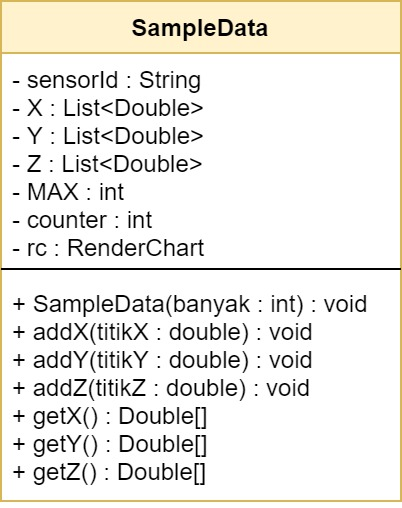
\includegraphics[scale=0.35]{Gambar/Controller Package/Controller-sampleData.jpg}
	\caption[Perancangan Kelas SampleData]{Perancangan Kelas SampleData}
	\label{fig:controller_sampleData} 
\end{figure}
Kelas ini digunakan untuk membuat sampel data. Kelas ini memiliki atribut-atribut sebagai berikut:
\begin{itemize}
    \item public double[] X;
    
    Atribut ini digunakan untuk menampung nilai x.
    
    \item public double[] Y;
    
    Atribut ini digunakan untuk menampung nilai y.
    
    \item public double[] Z;
    
    Atribut ini digunakan untuk menampung nilai z.
\end{itemize}

Metode-metode yang terdapat pada kelas ini adalah sebagai berikut:
\begin{itemize}
    \item public SampleData(int banyak);
    
    Metode ini digunakan sebagai konstruktor dari kelas SampleData.
    
    \item public void setX(double titikX);
    
    Metode ini digunakan sebagai setter dari atribut X.
    
    \item public void setY(double titikY);
    
    Metode ini digunakan sebagai setter dari atribut Y.
    
    \item public void setZ(double titikZ);
    
    Metode ini digunakan sebagai setter dari atribut Z.
    
\end{itemize}

\subsubsection{Kelas Sensor}
\begin{figure}[H] 
	\centering  
	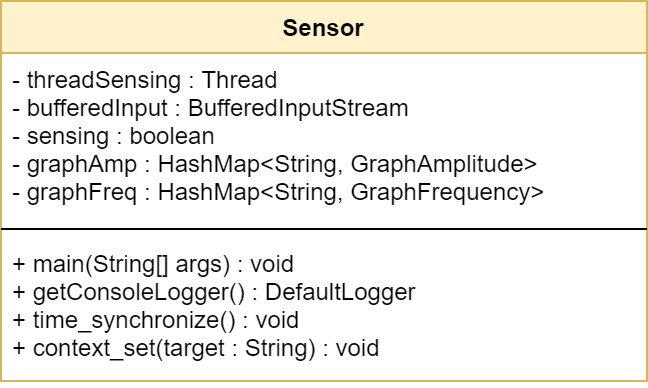
\includegraphics[scale=0.35]{Gambar/Controller Package/Controller-Sensor.jpg}
	\caption[Perancangan Kelas Sensor]{Perancangan Kelas Sensor}
	\label{fig:controller_sensor} 
\end{figure}
Kelas ini digunakan sebagai main class yang menerima input dari pengguna dan menampilkan output ke pengguna. Atribut-atribut yang terdapat pada kelas ini adalah sebagai berikut:

\begin{itemize}
    \item private static Thread threadSensing;
    
    Atribut ini digunakan untuk membuat thread baru yang bertujuan untuk menerima hasil sense dari sensor node saat dalam kondisi sensing.
    
    \item private static BufferedInputStream bufferedInput;
    
    Atribut ini digunakan untuk membaca input dari BaseStation.
    
    \item private static boolean sensing;
    
    Atribut ini digunakan sebagai penanda kondisi apakah SensorNode sedang melakukan sensing atau tidak.
    
\end{itemize}

Metode-metode yang terdapat pada kelas ini adalah sebagai berikut:

\begin{itemize}
    \item public static void main(String[] args);
    
    Metode ini digunakan sebagai metode main dari kelas ini.
    
    \item private static DefaultLogger getConsoleLogger();
    
    Metode ini digunakan untuk memunculkan tulisan pada console.
    
    \item private void time\_synchronize();
    
    Metode ini digunakan untuk mengatur dan memperbarui waktu pada BaseStation dengan waktu pada komputer pengguna.
    
    \item private void context\_set(String target);
    
    Metode ini digunakan untuk memilih context dari BaseStation.
\end{itemize}

\section{Perancangan Input dan Output}
Aplikasi ini menggunakan interface \textit{command line} untuk menerima input dari pengguna dan menampilkan keluaran dari aplikasi. Setiap input untuk aplikasi ini menggunakan tipe xdata \textit{integer}. Aplikasi ini akan menampilkan 4 pilihan fungsi \ref{fungsi_interaksi} dan pengguna dapat memasukan nilai dari 1 hingga 4 sebagai masukan untuk menjalankan fungsi tersebut. Berikut penjelasan perihal setiap masukan yang dapat dimasukkan oleh pengguna:
\begin{itemize}
    \item Masukan dengan nilai 1 merupakan fungsi "Check Online Node Status" yang digunakan untuk mengetahui status dari setiap node sensor dan melakukan penyamaan waktu yang ada di node sensor
    
    \item Masukan dengan nilai 2 merupakan fungsi "Start Sensing" yang digunakan untuk memberikan perintah \textit{sense} ke SensorNode dan menerima hasil sensing.
    
    \item Masukan dengan nilai 3 merupakan fungsi "Stop Sensing" yang digunakan untuk memeberikan perintah berhenti sensing pada node sensor
    
    \item Masukan dengan nilai 4 merupakan fungsi "Exit Program yang digunakan untuk memberhentikan program \textit{Controller} dan juga program pada \textit{SensorNode}
\end{itemize}

Jika pengguna memasukan fungsi selain "Stop Sensing" ketika \textit{SensorNode} melakukan sensing, maka \textit{Controller} akan menampilkan pesan "STILL SENSING.. USE OPTION "3" TO STOP IT!".

\section{Perancangan Antar Muka Untuk Visualisasi}
\begin{figure}[H] 
	\centering  
	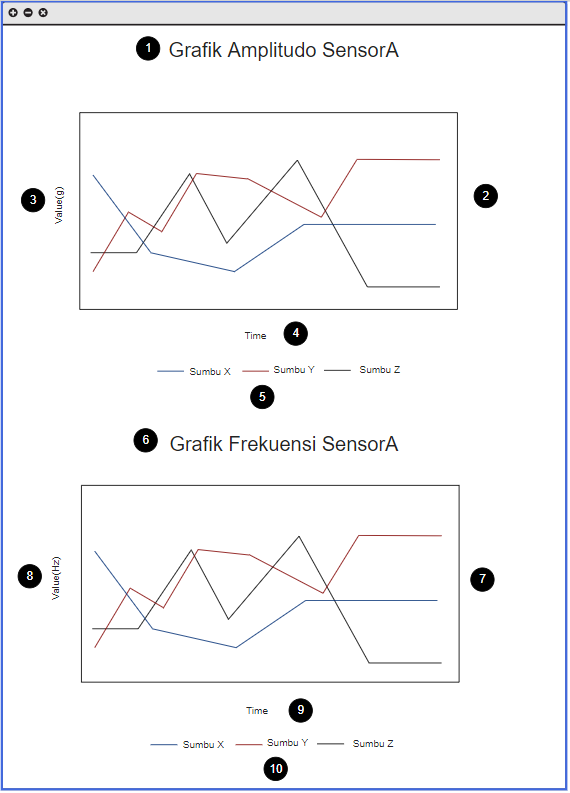
\includegraphics[scale=1]{Gambar/tampilanData.PNG}
	\caption[Rancangan antar muka tampilan grafik amplitudo dan frekuensi sensor]{Rancangan antar muka tampilan grafik amplitudo dan frekuensi sensor}
	\label{fig:tampilandata} 
\end{figure}

Keterangan Gambar:
\begin{itemize}
    \item Nomor 1 : Judul dari tampilan amplitudo sensor
    \item Nomor 2 : Grafik yang menampilkan hasil Amplitudo dari setiap sumbu
    \item Nomor 3 : Label 'Value(g)' yang dinyatakan untuk besarnya amplitudo
    \item Nomor 4 : Label 'Time' yang digunakan untuk menyatakan waktu
    \item Nomor 5 : Keterangan plot pada grafik yang ditampilkan
    \item Nomor 6 : Judul dari tampilan frekuensi sensor
    \item Nomor 7 : Grafik yang menampilkan hasil Frekuensi dari setiap sumbu
    \item Nomor 8 : Label 'Value(Hz)' yang dinyatakan untuk besarnya Frekuensi
    \item Nomor 9 : Label 'Time' yang digunakan untuk menyatakan waktu
    \item Nomor 10 : Keterangan plot pada grafik yang ditampilkan
\end{itemize}

\section{Perancangan Pseudocode Aplikasi}
\subsection{Start Chart}
Kelas \textit{Start Chart} ini berfungsi untuk membuat window hasil grafik yang akan ditampilkan ke \textit{user}. Metode yang digunakan untuk menampilkan grafik ini adalah \textit{getScene()} dan metode yang digunakan untuk menyimpan data hasil sensing dan nilai FFT adalah \textit{addData()}. Objek kelas dari StartChart akan digunakan ke abstract kelas yang bertujuan untuk menampilkan nilai amplitudo dan frekuensi. Berikut adalah \textit{pseudocode} dari metode \textit{getScene()} dan \textit{addData()}:

\begin{itemize}

    \item Pseudocode \textit{getScene()}
    
    \begin{algorithm}
        \caption{getScene}
        \label{alg:getScene}
        \begin{algorithmic}[1]
            \State \textbf{Input :} - 
            \State \textbf{Output :} Scene
            \Function{getScene}{}
                \State charts $\leftarrow$ new ChartAmplitude(getSample(), getData(), sensorId)
                \State getSample.setRender(charts.get(0)
                \State charts $\leftarrow$ new ChartFrequency(getSample(), getData(), sensorId)
                \State getSample.setRender(charts.get(1)
                \State ap $\leftarrow$ AnchorPane
                \State i $\leftarrow$ 0
                \State height $\leftarrow$ 400
                \State width $\leftarrow$ 600
                \For{charts in chart}
                    \State lc $\leftarrow$ LineChart
                    \State lc $\leftarrow$ charts.getChart()
                    \State lc.relocate(0, height*i)
                    \State i++
                    \State ap.getChildren.add(LineChart)
                    \State lc.setMinSize(width, height)
                    \State lc.setMaxXize(width, height)
                \EndFor
                \State return new Scene(ap, width, i*height);
            \EndFunction
        \end{algorithmic}
    \end{algorithm}
    
    \pagebreak
    \item Pseudocode \textit{addData()}
    
    \begin{algorithm}
        \caption{addData()}
        \label{alg:addData}
        \begin{algorithmic}[1]
            \State \textbf{Input :} String[]
            \State \textbf{Output :} -
            \Function{addData}{}
                \If{hasil[0].charAt(0) $\leftarrow$ 2}
                    \State getSample().addX(Double.parseDouble(hasil[1]))
                    \State getSample().addY(Double.parseDouble(hasil[2]))
                    \State getSample().addZ(Double.parseDouble(hasil[3]))
                    
                    \State computeFFT $\leftarrow$ FFT
                    \State computeFFT.convertComplex()
                    \State tempRes1 $\leftarrow$ computeFFT.fft(computeFFT.xComplex)
                    \State tempRes2 $\leftarrow$ computeFFT.fft(computeFFT.yComplex)
                    \State tempRes3 $\leftarrow$ computeFFT.fft(computeFFT.zComplex)
                    
                    \State df $\leftarrow$ DecimalFormat("*.****")
                    \For{i to tempRes1.length}
                        \State t1 $\leftarrow$ t1 + tempRes1[i].absolute()
                        \State t2 $\leftarrow$ t2 + tempRes2[i].absolute()
                        \State t3 $\leftarrow$ t3 + tempRes3[i].absolute()
                    \EndFor
                    
                    \State t1 $\leftarrow$ t1 / tempRes1.length
                    \State t2 $\leftarrow$ t2 / tempRes2.length
                    \State t3 $\leftarrow$ t3 / tempRes3.length
                    
                    \State getData().setX(Double.parseDouble(df.format(t1)))
                    \State getData().setY(Double.parseDouble(df.format(t2)))
                    \State 
                    getData().setZ(Double.parseDouble(df.format(t3)))
                \EndIf
            \EndFunction
        \end{algorithmic}
    \end{algorithm}
\end{itemize}

\subsection{ChartAmplitude \& ChartFrequency}
Kelas ini berfungsi untuk menampilkan LineChart yang akan ada pada window dari kelas StartChart. Kedua kelas ini cara mengimplementasikannya hampir sama satu sama lain, metode yang digunakan untuk menampilkan LineChart pada kelas tersebut adalah \textit{getChart()}. Terdapat juga metode \textit{render()} yang digunakan untuk melakukan \textit{update} nilai pada sumbu X dan Y pada \textit{Line Chart}. Berikut adalah pseudocode dari metode \textit{getChart()} dan \textit{render()} dari kelas ChartAmplitude dan ChartFrequency.

\begin{itemize}
    \pagebreak
    \item Pseudocode getChart() (ChartAmplitude)
    \begin{algorithm}
        \caption{getChart()}
        \label{alg:getChartAmplitude}
        \begin{algorithmic}[1]
            \State \textbf{Input :} -
            \State \textbf{Output :} LineChart
            \Function{getChart()}{}
                \State final x $\leftarrow$ CategoryAxis()
                \State final y $\leftarrow$ NumberAxis()
                
                \State x.setLabel("Time")
                \State x.setAnimated(false)
                
                \State y.setLabel("Value(g)")
                \State y.setAnimated(false)
                
                \State lineChart $\leftarrow$ LineChart<>(x,y)
                \State linechart.setAnimated(false);
                
                \State series1.setName("Sumbu X")
                \State series2.setName("Sumbu Y")
                \State series3.setName("Sumbu Z")
                
                \State lineChart.getData().add(series1)
                \State lineChart.getData().add(series2)
                \State lineChart.getData().add(series3)
                
                \State render()
                \State return lineChart
            \EndFunction
        \end{algorithmic}
    \end{algorithm}
    
    \item Pseudocode getChart() (ChartFrequency)
    \begin{breakablealgorithm}
        \caption{getChart()}
        \label{alg:getChartFrequency}
        \begin{algorithmic}[1]
            \State \textbf{Input :} -
            \State \textbf{Output :} LineChart
            \Function{getChart()}{}
                \State final x $\leftarrow$ CategoryAxis()
                \State final y $\leftarrow$ NumberAxis()
                
                \State x.setLabel("Time")
                \State x.setAnimated(false)
                
                \State y.setLabel("Value(Hz)")
                \State y.setAnimated(false)
                
                \State lineChart $\leftarrow$ LineChart<>(x,y)
                \State linechart.setAnimated(false);
                
                \State series1.setName("Sumbu X")
                \State series2.setName("Sumbu Y")
                \State series3.setName("Sumbu Z")
                
                \State lineChart.getData().add(series1)
                \State lineChart.getData().add(series2)
                \State lineChart.getData().add(series3)
                
                \State render()
                \State return lineChart
            \EndFunction
        \end{algorithmic}
    \end{breakablealgorithm}
    
    \pagebreak
    \item Pseudocode render() (ChartAmplitude)
    \begin{algorithm}
        \caption{render()}
        \label{alg:renderAmplitude}
        \begin{algorithmic}[1]
            \State \textbf{Input :} -
            \State \textbf{Output :} - 
            \Function{render()}{}
                \State Platform.runlater(new Runnable()){}
                \Function{run()}{}
                    \State now $\leftarrow$ Date()
                    \State lineChart.setTitle("Grafik Amplitudo "+sensorId)
                    \State series1.getData().add(new XYChart.Data<>(SimpleDateFormat.format(now), getX()))
                    \State series2.getData().add(new XYChart.Data<>(SimpleDateFormat.format(now), getY()))
                    \State series3.getData().add(new XYChart.Data<>(SimpleDateFormat.format(now), getZ()))
                    
                    \If{series1.getData().size() $>$ WINDOW\_SIZE}
                        \State series1.getData().remove(0)
                        \State series2.getData().remove(0)
                        \State series3.getData().remove(0)
                    \EndIf
                \EndFunction
            \EndFunction
        \end{algorithmic}
    \end{algorithm}

    \item Pseudocode render() (ChartFrequency)
    \begin{breakablealgorithm}
        \caption{render()}
        \label{alg:renderFrequency}
        \begin{algorithmic}[1]
            \State \textbf{Input :} -
            \State \textbf{Output :} - 
            \Function{render()}{}
                \State Platform.runlater(new Runnable()){}
                \Function{run()}{}
                    \State now $\leftarrow$ Date()
                    \State lineChart.setTitle("Grafik Frekuensi "+sensorId)
                    \State series1.getData().add(new XYChart.Data<>(SimpleDateFormat.format(now), dataFrequency.X()))
                    \State series2.getData().add(new XYChart.Data<>(SimpleDateFormat.format(now), dataFrequency.Y()))
                    \State series3.getData().add(new XYChart.Data<>(SimpleDateFormat.format(now), dataFrequency.Z()))
                    
                    \If{series1.getData().size() $>$ WINDOW\_SIZE}
                        \State series1.getData().remove(0)
                        \State series2.getData().remove(0)
                        \State series3.getData().remove(0)
                    \EndIf
                \EndFunction
            \EndFunction
        \end{algorithmic}
    \end{breakablealgorithm}
\end{itemize}

\subsection{Controller}
Kelas Controller memiliki fungsi untuk menyimpan hasil sensing yang dilakukan oleh sensor dan melakukan algoritma FFT. Metode yang ada pada kelas ini adalah FFT() dan \textit{bitReverse()}. Berikut adalah pseudocode dari metode FFT() dan \textit{bitReverse()}

\begin{itemize}
    \pagebreak
    \item Pseusodocde \textit{bitReverse()}
    
    \begin{algorithm}
        \caption{bitReverse()}
        \label{alg:bitReverse}
        \begin{algorithmic}[1]
            \State \textbf{Input :} n, bits
            \State \textbf{Output :} int 
            \Function{bitReverse(n, bits)}{}
                \If{n $==$ 0}
                    \State return 0;
                \EndIf
                \State temp $\leftarrow$ n menjadi binaryString
                \If{panjang temp $<$ bits}
                    \State k $\leftarrow$ bits - panjang temp
                    \While{i $\leftarrow$} 0 to k, i $\leftarrow$ i+1
                        temp $\leftarrow$ "0" + temp
                    \EndWhile
                \EndIf
                \State res $\leftarrow$ 0
                \For{i $\leftarrow$ panjang temp-1 ; i$>=$0; i $\leftarrow$ i-1}
                    \If{huruf ke i dari temp $==$ '1'}
                        res $\leftarrow$ res + $2^i$
                    \EndIf
                \EndFor
                \State return res
            \EndFunction
        \end{algorithmic}
    \end{algorithm}
    
    \item Pseudocode \textit{FFT()}
    
    \begin{breakablealgorithm}
        \caption{FFT()}
        \label{alg:fft}
        \begin{algorithmic}[1]
            \State \textbf{Input :} input
            \State \textbf{Output :} Complex[] 
            \Function{FFT(input)}{}
                bits $\leftarrow$ \textit{Logpanjanginput/log2}
                orderFinal $\leftarrow$ inisialisasi array Complex sebesar panjang input
                \For{i $\leftarrow$ 0; i$<$ panjang input;i++}
                    order $\leftarrow$ bitReverse(i,bits)
                    orderFinal[i] $\leftarrow$ input[order]
                \EndFor
                \For{i $\leftarrow$ 2; j$<=$panjang orderFinal; i $\leftarrow$ i x 2}
                    \For{j $\leftarrow$ 0; j$<$panjang orderFinal; j$\leftarrow$ j+i}
                        \For{k$\leftarrow$0; k$<$i/2; k$\leftarrow$k+1}
                            \State awal $\leftarrow$ orderFinal[j+k]
                            \State akhir $\leftarrow$ orderFinal[j+k+(i/2)]
                            \State weight $\leftarrow$ (-2$\pi$k)/i
                            \State exponential $\leftarrow$ new Complex(cos(weight), sin(weight)).multiplication(akhir)
                            \State orderFinal[j+k] $\leftarrow$ awal tambah exponential
                            \State orderFinal[j+k+(i/2)] $\leftarrow$ awal kurang exponential
                        \EndFor
                    \EndFor
                \EndFor
                \State return orderFinal
            \EndFunction
        \end{algorithmic}
    \end{breakablealgorithm}
    
\end{itemize}
    
    
    
    


